\chapter{Další možné využití}

%Původní nápad -- proč je použit ohebný pásek? 		
Mým původním nápadem bylo, že mojí ročníkovou prací bude výroba plnohodnotné lampičky, počítaje jak elektrotechnickou část tak tu designovou. Z toho bohužel sešlo z časových důvodů, a tak tu teoreticky proberu designovou část. 
Důvod, proč jsem později zaměnila pevní LED pásek za ohebný, byl ten, že původně jsem měla nápad, že ohebný LED pásek by se dal lépe schovat do předem připravené plastové žárovky. 
Žárovka by byla tvořená z~průhledné Křišťálové pryskyřice tzv. epoxy resin\cite{epoxyresin}, což je čirá odlévací tekutina používající se jak na umělecké, tak technické účely. Z toho sešlo kvůli problémům zvládnutí této techniky a nedostatku času. 



%Další nápady -- Více světel bez/drátově propojená. 		
Také by bylo možné naprogramovat více \textit{ESP32-DevkitC} s LED, které by se mohly navzájem propojit, ať už dráty, anebo bezdrátově. V bezdrátové verzi vidím víc výhod, ale zase by mohl být problém s dosahem a dálkou od ovládacího zařízení. 
Na LED pásky by se dalo vyrobit více tzv. žárovek tím, že by se podle předem vytvořeného originálu vyrobila forma na~silikon a ta by se následně opakovaně použila na odlití Epoxidové pryskyřice. Každé světlo by mělo tzv. {\em základnu}, která by byla buď vytvořená z dřevěných desek přesně vypálených na~laseru, anebo by se vytiskl plastový obal na 3D tiskárně. Tato možnost se mi asi líbí nejvíc.

	
%todo laser odkaz??? 3d tiskárna odkaz?		

S trochou snahy, kreativity a hodně práce by se z tohoto prototypu mohla stát i sada pro~začínající programátory a elektrotechniky, protože práce na mém LED prototypu pokryje jak pájení a práci s elektronickými součástkami, tak programování, kdy člověk může buď už~předem naprogramovaný program stáhnout z internetu, nebo si ho naprogramovat a upravit podle sebe. 

Ráda bych tuto ročníkovou práci ukončila s myšlenkou, že můj prototyp svítících LED světel má kreativní využití ve všech směrech a je jen na konstruktérovi, jak bude tento nápad chtít využít. 


%   \begin{figure}[htbp]
%	\centering
%	\begin{minipage}[b]{0.5\textwidth}
%		\centering
%		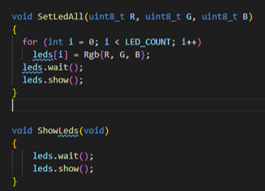
\includegraphics[width=0.75\textwidth]{img/015 img/definovane-funkce.png}
%		\caption{Funkce}
%		%		\label{fig:gear-sketch1}
%	\end{minipage}
%	\qquad
%	\begin{minipage}[b]{0.4\textwidth}
%		\centering
%		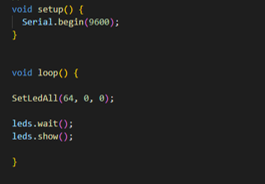
\includegraphics[width=1\textwidth]{img/015 img/Program1-červená.png}
%		\caption{Program}
%		%		\label{fig:gear-sketch2}
%	\end{minipage}
%\end{figure}
